\begin{frame}{Running on Piz Daint}{The job scheduler}
  Piz Daint uses native SLURM for running jobs on the compute nodes.
  There are three ways of submitting a job:
  \vspace\baselineskip
  \begin{enumerate}
  \item Interactively from the login nodes using the \texttt{srun} command.
  \item By submitting a job script using the \texttt{sbatch} command.
  \item By pre-allocating resources using the \texttt{salloc} command.
  \end{enumerate}
\end{frame}

\begin{frame}[fragile]{Running on Piz Daint}{Using the \texttt{srun} command}
  Necessary and useful options:
  \begin{itemize}
  \item \texttt{-C gpu}: requests allocation on the hybrid (GPU) nodes (required)
  \item \texttt{--reservation=summer\_school}
    \begin{itemize}
    \item 64 nodes valid until Jul.\ 25 @ 13:00.
    \end{itemize}
  \item \texttt{-N 2}: number of compute nodes (default is 1)
  \item \texttt{-n 2}: number of MPI tasks (default is 1)
  \item \texttt{-t 5}: maximum duration of the job (default is 30min)
    \begin{itemize}
    \item Allows to get an allocation quicker
    \item Job will be killed if time limit is reached
    \item Maximum time slot for a job is 24h
    \end{itemize}
  \end{itemize}
  More on \url{https://user.cscs.ch/access/running}
\end{frame}

\begin{frame}[fragile]{Running on Piz Daint}{Using the \texttt{srun} command}
  {
    \centering
    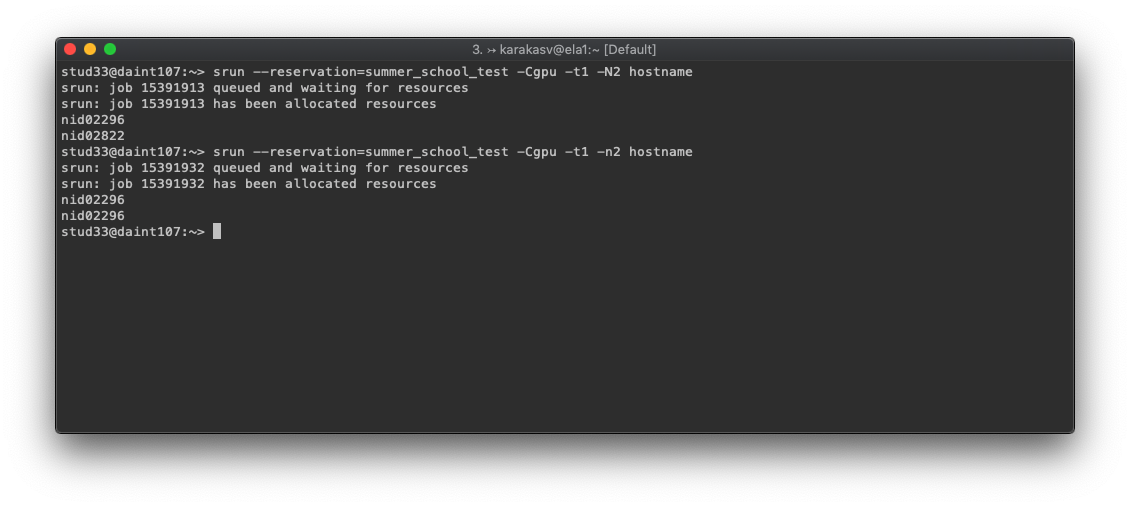
\includegraphics[width=\textwidth]{srun_hostname.png}
  }
\end{frame}

\begin{frame}[fragile]{Running on Piz Daint}{Using the \texttt{sbatch} command}
  {
    \centering
    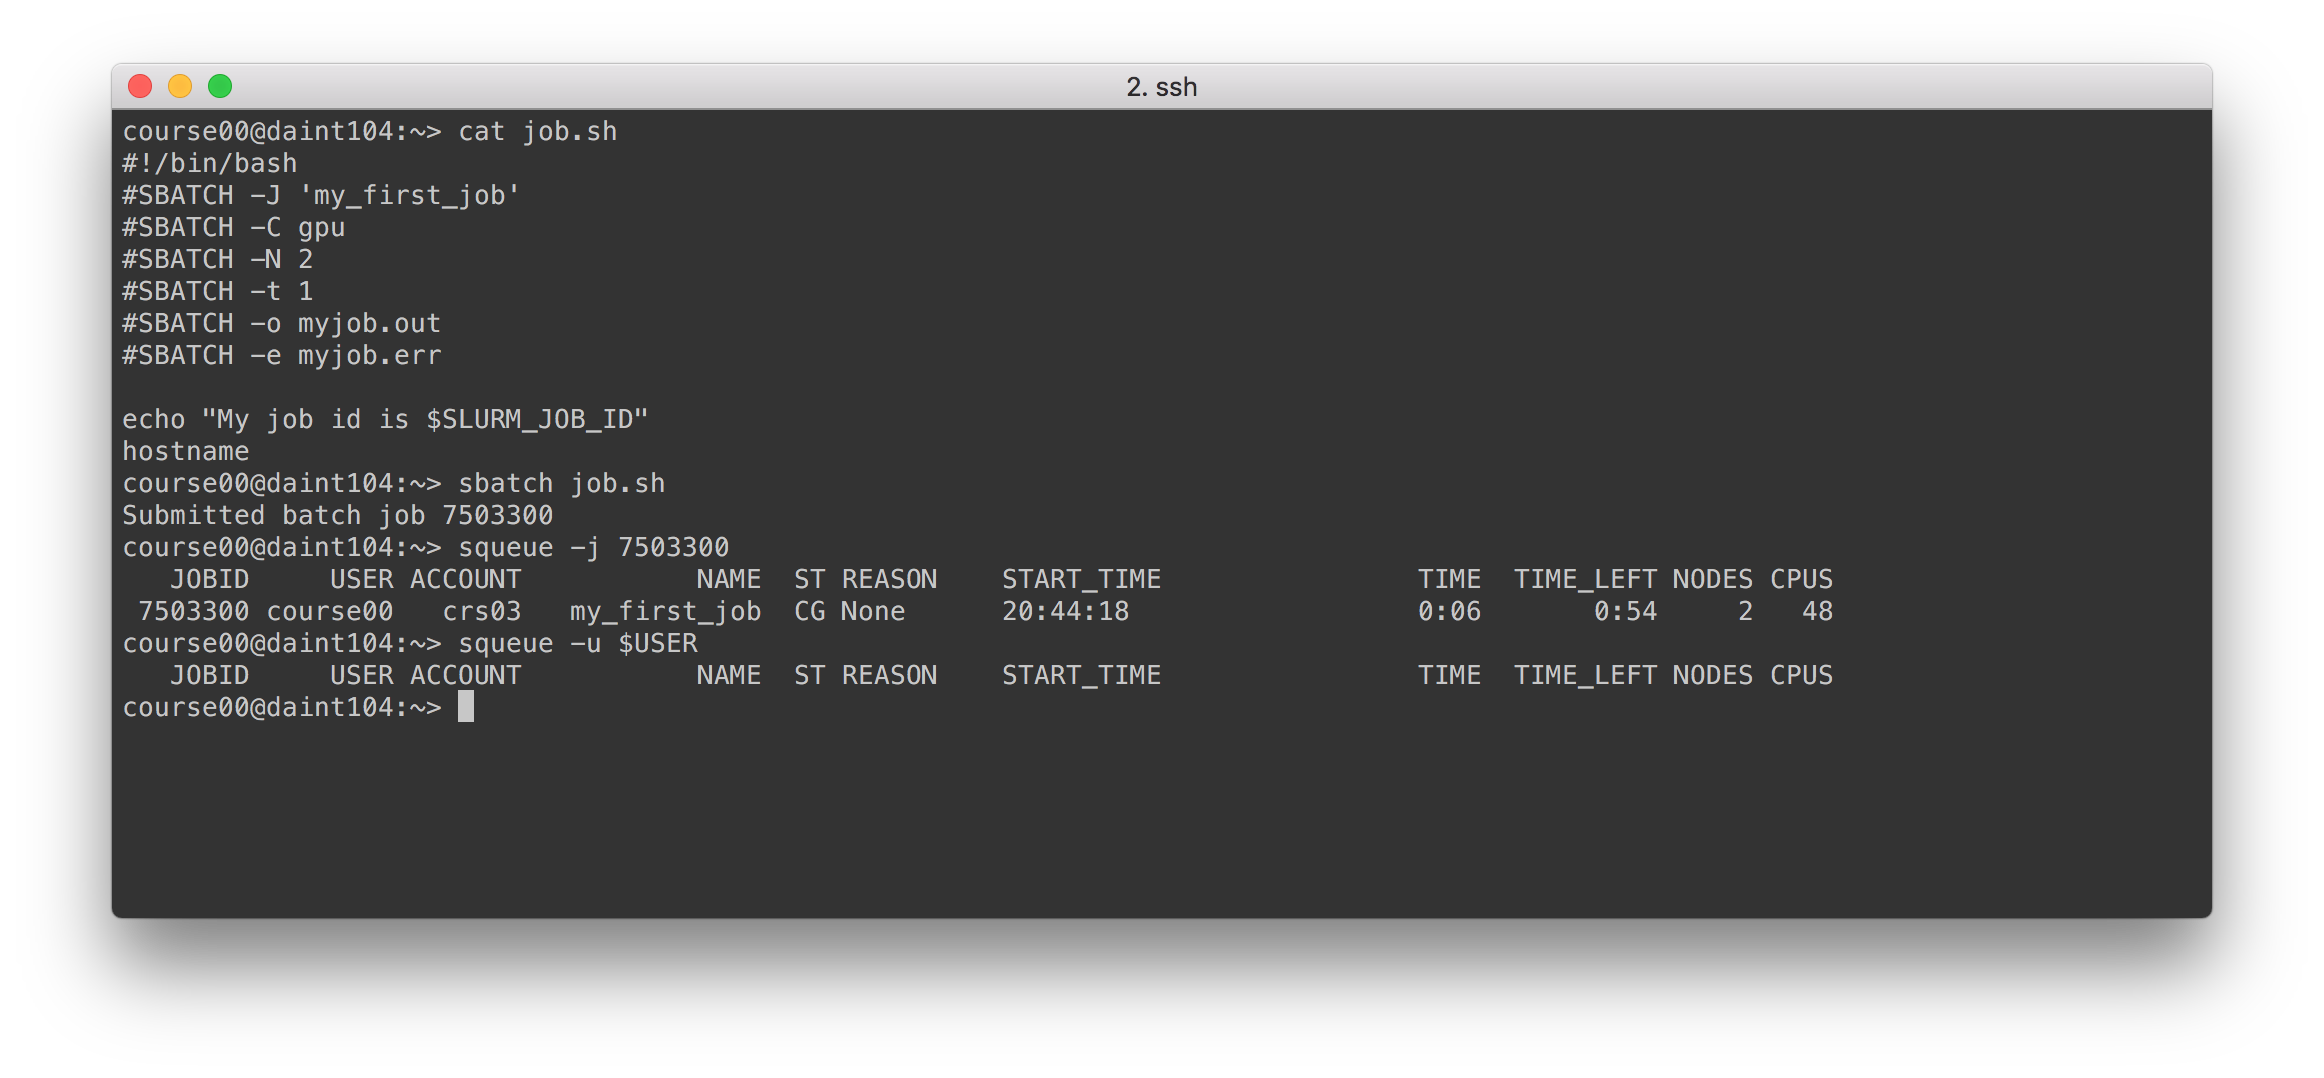
\includegraphics[width=\textwidth]{sbatch_hostname.png}
  }
\end{frame}


\begin{frame}[fragile]{Running on Piz Daint}{Using the \texttt{sbatch} command -- Examinining the output}
  {
    \centering
    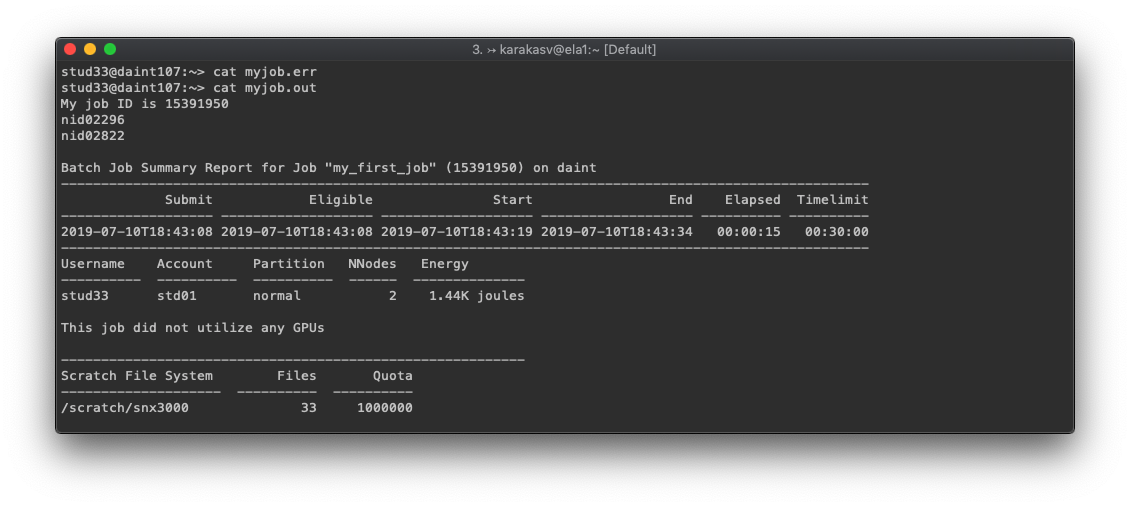
\includegraphics[width=\textwidth]{sbatch_hostname_output.png}
  }
\end{frame}

\begin{frame}[fragile]{Running on Piz Daint}{Using the \texttt{salloc} command}
  {
    \centering
    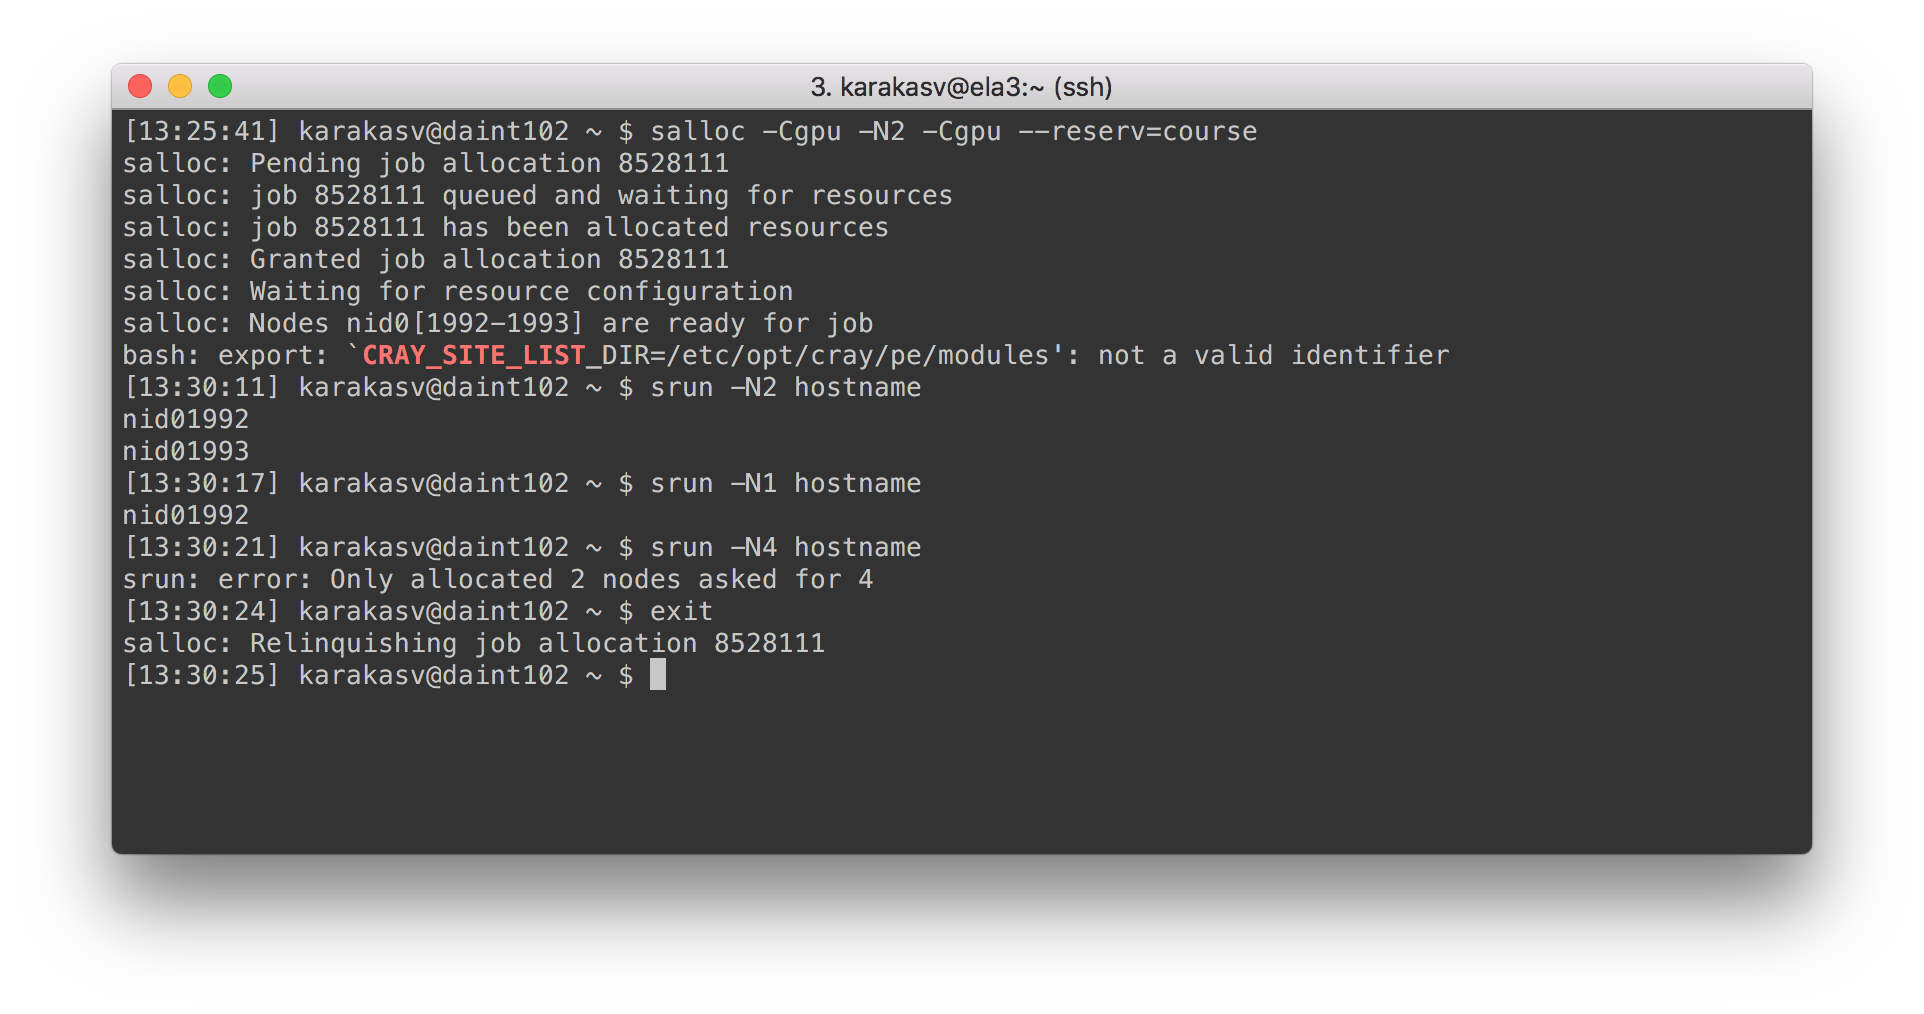
\includegraphics[width=\textwidth]{salloc_hostname.png}
  }
\end{frame}

\begin{frame}{Running on Piz Daint}{Other useful commands}
  \begin{itemize}
  \item \texttt{squeue [OPTIONS]}: Check the status of the system job queue
    \begin{itemize}
    \item Useful options: \texttt{-u [USERNAME]}, \texttt{-j [JOBID]}
    \end{itemize}
  \item \texttt{scancel [JOBID]}: Cancel a job
  \item \texttt{scontrol}: Detailed information about partitions, reservations,
    computing nodes etc.
  \end{itemize}
\end{frame}

\begin{frame}{Running on Piz Daint}{Other useful commands}
  {
    \centering
    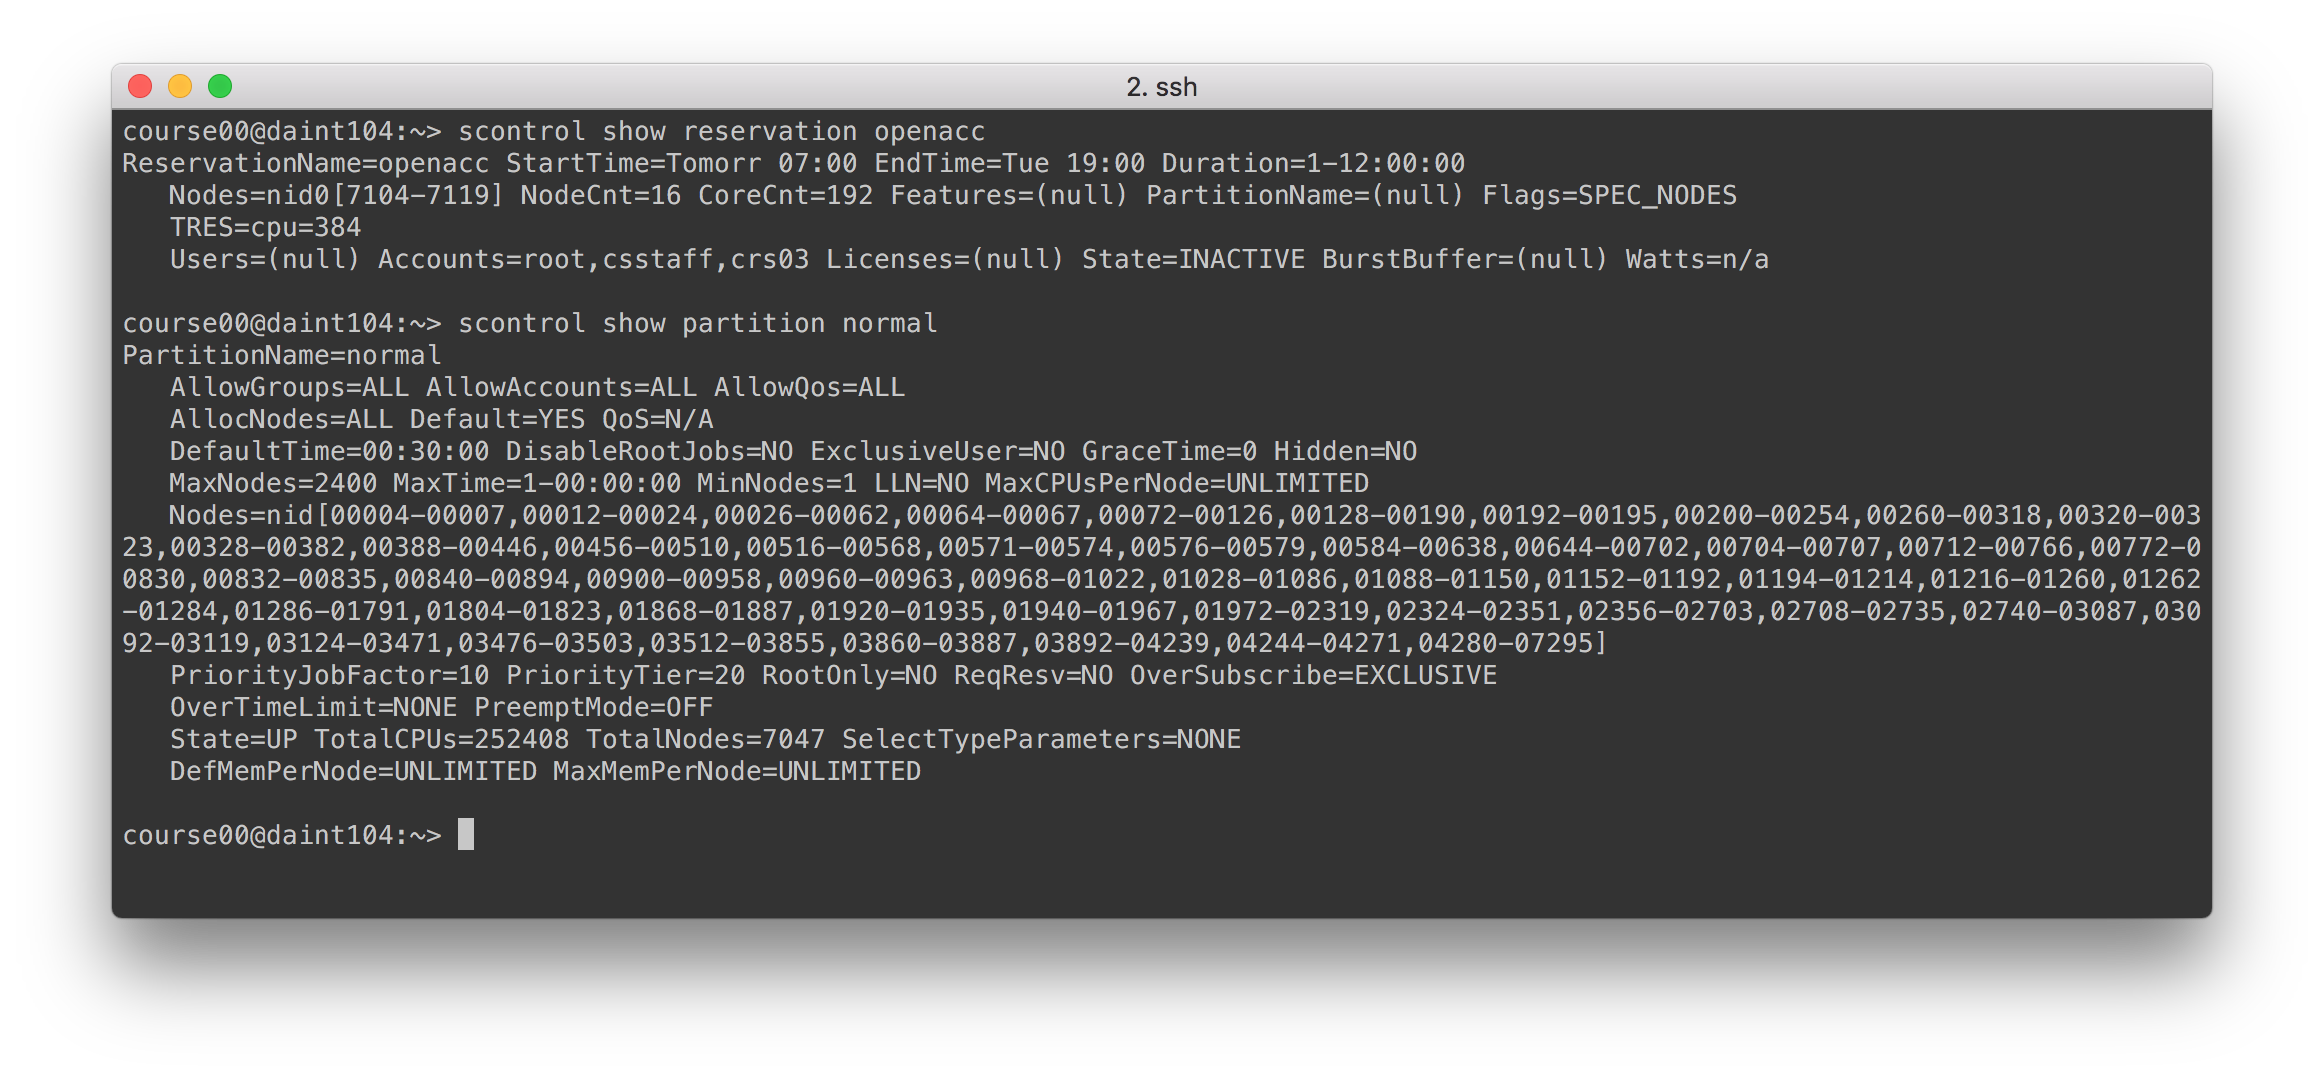
\includegraphics[width=\textwidth]{scontrol.png}
  }
\end{frame}
